\ifnotes
\else
  \PassOptionsToClass{handout}{beamer}
\fi

\documentclass[10pt,t]{beamer}

\usetheme{metropolis} % use metropolis theme

\usepackage{solarized}            % use solarized themed listings
\usepackage{appendixnumberbeamer} % do not number appendix frames
\usepackage[scale=3]{ccicons}     % creative commons icons

% fix-up the handling of the notes pages
\ifnotes
  \hypersetup{final}
  \usepackage{pgfpages}
  \setbeamertemplate{note page}[plain]
  \setbeameroption{show notes on second screen=right}
\fi

%-------------------------------------------------------------------------------

\usepackage{tabularx}
\usepackage{tikz}
\usetikzlibrary{decorations.pathreplacing}

\title{C programming language}
\date{}
\author{Jeremy Iverson}
\institute{College of Saint Benedict \& Saint John's University}
\begin{document}
  \maketitle

  \begin{frame}{origins}
    \vspace{3ex}
    \begin{columns}
      \begin{column}{.38425\textwidth}
        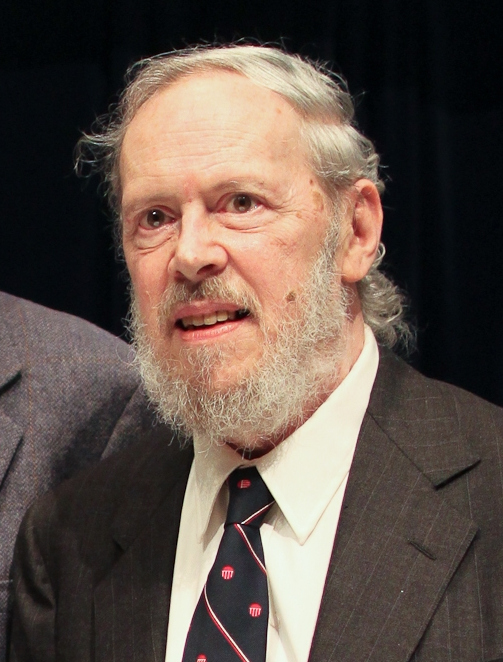
\includegraphics[width=\textwidth]{Dennis_Ritchie_2011.jpg}\\
        \hfill \tiny{\href{https://en.wikipedia.org/wiki/Dennis\_Ritchie\#/media/File:Dennis\_Ritchie\_2011.jpg}{Dennis~Ritchie~in~2011}~/~\href{http://creativecommons.org/licenses/by-sa/2.0}{CC~BY~2.0}}
      \end{column}
      \begin{column}{.51575\textwidth}
        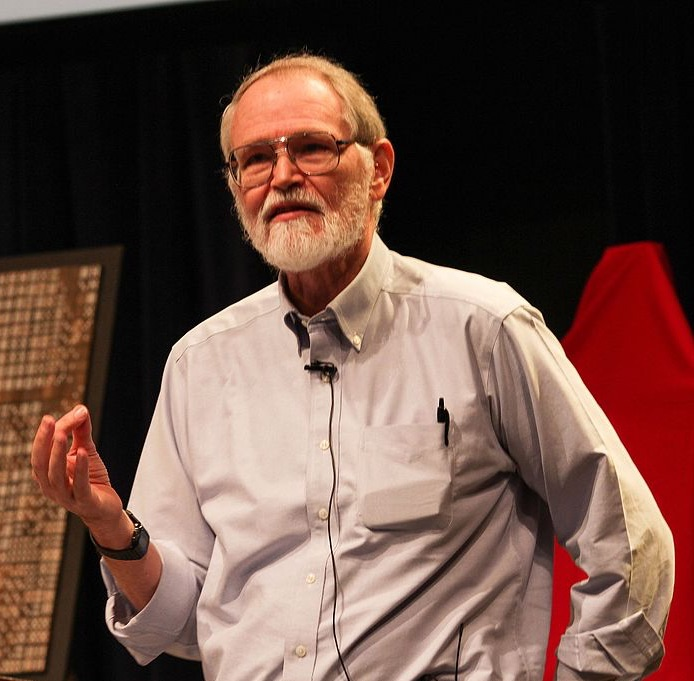
\includegraphics[width=\textwidth]{Brian_Kernighan_in_2012.jpg}\\
        \hfill \tiny{\href{https://en.wikipedia.org/wiki/Brian\_Kernighan\#/media/File:Brian\_Kernighan\_in\_2012\_at\_Bell\_Labs\_1.jpg}{Brian~Kernighan~in~2012}~/~\href{http://creativecommons.org/licenses/by-sa/2.0}{CC~BY~2.0}}
      \end{column}
    \end{columns}

    \note{
      \begin{itemize}
        \item Dennis Ritchie and Brian Kernighan creators of C circa 1972
      \end{itemize}
    }
  \end{frame}

  \begin{frame}{comparison}
    \begin{center}
      \begin{tabularx}{.8\textwidth}{XX}
        \hline
        \textbf{Java} & \textbf{C}\\
        \hline
        object-oriented & procedural\\
        interpreted & compiled\\
        \texttt{String} & \texttt{char} array\\
        condition (\texttt{boolean}) & condition (\texttt{int})\\
        garbage-collected & no memory management\\
        references & pointers\\
        exceptions & error codes\\
        \hline
      \end{tabularx}
    \end{center}

    \note{
      \begin{itemize}
        \item in Java, everything is a method that is called on an object
        \item in C, everything is a function
      \end{itemize}
      \begin{itemize}
        \item in Java, source code is compiled to byte code, which is then
          interpreted by Java VM
        \item in C, source code is compiled into binary machine code
      \end{itemize}
      \begin{itemize}
        \item in Java, String is a class
        \item in C, a string is just an array of \texttt{char} values which ends
          with the \texttt{char~'\textbackslash0'}
      \end{itemize}
      \begin{itemize}
        \item in Java, the Java VM takes care of deallocating memory used
        \item in C, any memory you allocate, you must also deallocate
      \end{itemize}
    }
  \end{frame}

  \begin{frame}[fragile]{hello, world}
    \begin{codeblock}
    ###include## $$<stdio.h>$$

    int main() {
      printf([["hello, world]]%%\n%%[["]]);
      return $$0$$;
    }
    \end{codeblock}

    \begin{termblock}
    $ gcc -o helloworld helloworld.c
    $ ./helloworld
    hello, world
    \end{termblock}

    \note{
      \begin{itemize}
        \item The tradition of using the phrase "Hello, world!" as a test
          message was influenced by an example program in the seminal book
          \emph{The C Programming Language}
      \end{itemize}
    }
  \end{frame}

  \begin{frame}[fragile]{conditions}
    \begin{itemize}
      \item under what conditions will each of the following be execute?
    \end{itemize}
    \begin{codeblock}
    if (x) {
      /* ??? */
    }
    if (x-y) {
      /* ??? */
    }
    if (x=y) {
      /* ??? */
    }
    \end{codeblock}

    \note{
      \begin{itemize}
        \item x != 0
        \item x != y
        \item y != 0
      \end{itemize}
    }
  \end{frame}

  \begin{frame}{add evens}
    \begin{itemize}
      \item create program called \texttt{add\_even.c} that adds all the even
        numbers between 1 and 100 and prints the sum
    \end{itemize}
  \end{frame}

  \begin{frame}[fragile]{cli}
    \begin{codeblock}
    ###include## $$<stdio.h>$$

    int main(int argc, char * argv[]) {
      printf([["(]]%%%d%%[[) ]]%%%s%%[[:]]%%%s\n%%[["]], argc, argv[$$0$$],
        argv[$$1$$]);
      return $$0$$;
    }
    \end{codeblock}

    \begin{itemize}
      \item modify \texttt{add\_even.c} to get maximum value from the
        command-line instead of hard-coded as 100
    \end{itemize}
  \end{frame}

  \begin{frame}[fragile]{printf / scanf}
    \begin{itemize}
      \item \texttt{printf()} interprets variables and prints character
        representations to standard out (usually the terminal)
      \item \texttt{scanf()} scans characters from standard in (usually the
        terminal) and interprets them for storage in variables
    \end{itemize}

    \begin{codeblock}
    ###include## $$<stdio.h>$$

    int main() {
      int i;
      scanf([["]]%%%d%%[["]], &i);
      return $$0$$;
    }
    \end{codeblock}

    \note{
      \begin{itemize}
        \item scanf requires you to pass the address of the variable, so that
          its value can be changed
      \end{itemize}
    }
  \end{frame}

  \begin{frame}[fragile]{echo}
    \begin{itemize}
      \item modify \texttt{helloworld.c} to ask user for an input and then print
        it back
      \item change its name to \texttt{echo.c}
    \end{itemize}

    \begin{termblock}
    $ ./echo
    Enter a string to echo: hello, world
    hello,
    \end{termblock}

    \note{
      \begin{itemize}
        \item why did it print \texttt{hello,} instead of \texttt{hello, world}?
      \end{itemize}
    }
  \end{frame}

  \begin{frame}[fragile]{pointers}
    \begin{itemize}
      \item a pointer is a variable whose value is a memory address
    \end{itemize}
    \begin{codeblock}
    int   i  = $$0x1A$$;
    int * ip = &i;
    \end{codeblock}
    \begin{itemize}
      \item \texttt{\&i} evaluates to the address where the variable \texttt{i}
        is stored in memory
      \item \texttt{i} is an \texttt{int}, so \texttt{ip} is a \emph{pointer} to
        an \texttt{int}
    \end{itemize}

    \hspace{8pt}%
    \begin{tikzpicture}[font=\ttfamily,noname/.style={text height=1.5ex, text depth=.25ex, text centered, minimum height=3em}]
      \node[noname] at (-1.3,.3) {\textbf{0x000012A0}};
      \foreach \x in {0,.6,...,2.4}
        \draw (\x,0) rectangle ++(.6,.6);
      \draw[bg, ultra thick] (-.1,.6) -- ++(3.2,0);
      \foreach [count=\i,evaluate=\i as \x using .3+(\i-1)*.6] \c in {00,00,00,1A}
        \node[noname] at (\x,.3) {\c};
      \draw[decoration={brace,mirror,raise=5pt},decorate] (2.4,0) -- node[right=6pt] {i} ++(0,.6);

      \node[noname] at (-1.3,-.7) {\textbf{0x????????}};
      \foreach \x in {0,.6,...,2.4}
        \draw (\x,-1) rectangle ++(.6,.6);
      \draw[bg, ultra thick] (-.1,-.4) -- ++(3.2,0);
      \foreach [count=\i,evaluate=\i as \x using .3+(\i-1)*.6] \c in {00,00,12,A0}
        \node[noname] at (\x,-.7) {\c};
      \draw[decoration={brace,mirror,raise=5pt},decorate] (2.4,-1) -- node[right=6pt] {ip} ++(0,.6);
    \end{tikzpicture}
  \end{frame}

  \begin{frame}[fragile]{pointers cont.}
    \begin{codeblock}
    printf([["0x]]%%%X\n%%[["]], i);    /* 0x1A */
    printf([["0x]]%%%#X\n%%[["]], &i);  /* 0x12A0 */
    printf([["0x]]%%%#X\n%%[["]], ip);  /* 0x12A0 */
    printf([["0x]]%%%#X\n%%[["]], &ip); /* 0x???????? */
    \end{codeblock}

    \note{
      \begin{itemize}
        \item so how can we use the pointer, \texttt{ip}, to access the value of
          \texttt{i}?
      \end{itemize}
    }
  \end{frame}

  \begin{frame}[fragile]{pointer dereference}
    \begin{itemize}
      \item \texttt{*ptr} will
        \begin{enumerate}
          \item treat the value of \texttt{ptr} as a memory address
          \item get the bytes of data located at that memory address
          \item interpret those bytes according to the type of pointer that
            \texttt{ptr} is
        \end{enumerate}
    \end{itemize}
    \begin{codeblock}
    printf([["0x]]%%%X\n%%[["]], *ip);   /* 0x1A */
    \end{codeblock}

    \begin{onlyenv}<2->
      \begin{itemize}
        \item \texttt{ip[X] = *(ip + X)}
      \end{itemize}
      \begin{codeblock}
    printf([["0x]]%%%X\n%%[["]], ip[0]); /* 0x1A */
      \end{codeblock}
    \end{onlyenv}

    \note{
      \begin{itemize}
        \item the C compiler is ''smart enough'' to ''know'' that \texttt{+ X}
          really means add \texttt{X * sizeof(*ip)} to \texttt{ip}
      \end{itemize}
    }
  \end{frame}

  \begin{frame}[fragile]{pointers cont.}
    \begin{codeblock}
    printf([["0x]]%%%X\n%%[["]], i);       /* 0x1A */
    printf([["0x]]%%%X\n%%[["]], *ip);     /* 0x1A */
    printf([["0x]]%%%X\n%%[["]], ip[$$0$$]);   /* 0x1A */
    printf([["0x]]%%%X\n%%[["]], *(ip+$$0$$)); /* 0x1A */
    printf([["0x]]%%%#X\n%%[["]], &i);     /* 0x12A0 */
    printf([["0x]]%%%#X\n%%[["]], ip);     /* 0x12A0 */
    printf([["0x]]%%%#X\n%%[["]], &ip);    /* 0x???????? */
    \end{codeblock}
  \end{frame}


  \begin{frame}[fragile]{pointers cont.}
    \begin{codeblock}
    char * cp = "hello, world";
    \end{codeblock}
    \begin{itemize}
      \item \texttt{cp} is a \emph{pointer} to a \texttt{char}
    \end{itemize}

    \vspace{-14pt}%
    \hspace{8pt}%
    \begin{tikzpicture}[font=\ttfamily,noname/.style={text height=1.5ex, text depth=.25ex, text centered, minimum height=3em}]
      \node[noname] at (-1.3,.3) {\textbf{0x00004C80}};
      \foreach \x in {0,.6,...,7.8}
        \draw (\x,0) rectangle ++(.6,.6);
      \draw[bg, ultra thick] (-.1,.6) -- ++(8.4,0);
      \foreach [count=\i,evaluate=\i as \x using .3+(\i-1)*.6] \c in {h,e,l,l,o,{,}, ,w,o,r,l,d,\textbackslash0}
        \node[noname] at (\x,.3) {\c};

      \node[noname] at (-1.3,-.7) {\textbf{0x????????}};
      \foreach \x in {0,.6,...,2.4}
        \draw (\x,-1) rectangle ++(.6,.6);
      \draw[bg, ultra thick] (-.1,-.4) -- ++(3.2,0);
      \foreach [count=\i,evaluate=\i as \x using .3+(\i-1)*.6] \c in {00,00,4C,80}
        \node[noname] at (\x,-.7) {\c};
    \end{tikzpicture}

    \vspace{-6pt}%
    \begin{codeblock}
    printf([["]]%%%c\n%%[["]], *cp);     /* h */
    printf([["]]%%%c\n%%[["]], cp[$$0$$]);   /* h */
    printf([["]]%%%c\n%%[["]], cp[$$4$$]);   /* o */
    printf([["]]%%%c\n%%[["]], *(cp+$$4$$)); /* o */
    printf([["]]%%%s\n%%[["]], cp);      /* hello, world */
    printf([["]]%%%s\n%%[["]], cp+7);    /* world */
    printf([["0x]]%%%#X\n%%[["]], cp);   /* 0x4C80 */
    printf([["0x]]%%%#X\n%%[["]], &cp);  /* 0x???????? */
    \end{codeblock}

    \note{
      \begin{itemize}
        \item why not say \texttt{cp} is a \emph{pointer} to a \texttt{char}
          array?
      \end{itemize}
    }
  \end{frame}

  \begin{frame}[fragile]{practice}
    \begin{codeblock}
    ###include## $$<stdio.h>$$

    void swap(int n1, int n2) {
      int tmp = n1;
      n1 = n2;
      n2 = tmp;
    }

    int main() {
      int v1 = $$11$$, v2 = $$77$$;
      printf([["BEFORE  v1=]]%%%d%%[[, v2=]]%%%d\n%%[["]], v1, v2);
      swap(v1, v2);
      printf([["AFTER  v1=]]%%%d%%[[, v2=]]%%%d\n%%[["]], v1, v2);
      return $$0$$;
    }
    \end{codeblock}

    \note{
      \begin{itemize}
        \item what's wrong with this program?
        \item fix the program so that it correctly swaps the two variables'
          values
      \end{itemize}
    }
  \end{frame}

  \begin{frame}[fragile]{heap memory}
    \begin{itemize}
      \item designate a block of memory to store value(s) of a particular
        data type
    \end{itemize}
    \begin{codeblock}
    int * ip = malloc($$100$$*sizeof(int));
    \end{codeblock}

    \hspace{8pt}%
    \begin{tikzpicture}[font=\ttfamily,noname/.style={text height=1.5ex, text depth=.25ex, text centered, minimum height=3em}]
      \node[noname] at (-1.3,.3) {\textbf{0x000063DA}};
      \foreach \x in {0,.6,...,7.2}
        \draw (\x,0) rectangle ++(.6,.6);
      \draw[bg, ultra thick] (-.1,.6) -- ++(8,0);
      \foreach [count=\i,evaluate=\i as \x using .3+(\i-1)*.6] \c in {r,@,!,X,t,v,9,1,S,?,{)},.}
        \node[noname] at (\x,.3) {\c};
      \node at (7.6,.3) {$\boldsymbol{\cdots}$};

      \node[noname] at (-1.3,-.7) {\textbf{0x????????}};
      \foreach \x in {0,.6,...,2.4}
        \draw (\x,-1) rectangle ++(.6,.6);
      \draw[bg, ultra thick] (-.1,-.4) -- ++(3.2,0);
      \foreach [count=\i,evaluate=\i as \x using .3+(\i-1)*.6] \c in {00,00,63,DA}
        \node[noname] at (\x,-.7) {\c};
    \end{tikzpicture}

    \begin{onlyenv}<2->
      \begin{itemize}
        \item release a block of memory back to system to be used elsewhere
      \end{itemize}
      \begin{codeblock}
    free(ip);
      \end{codeblock}
    \end{onlyenv}

    \note{
      \begin{itemize}
        \item allocates enough consecutive memory for 100 \texttt{int} values
      \end{itemize}
    }
  \end{frame}

  \begin{frame}[fragile]{heap memory cont.}
    \begin{codeblock}
    ip[$$0$$] = $$0x7$$; /* *ip = 0x7; */
    \end{codeblock}

    \hspace{8pt}%
    \begin{tikzpicture}[font=\ttfamily,noname/.style={text height=1.5ex, text depth=.25ex, text centered, minimum height=3em}]
      \node[noname] at (-1.3,.3) {\textbf{0x000063DA}};
      \foreach \x in {0,.6,...,7.2}
        \draw (\x,0) rectangle ++(.6,.6);
      \draw[bg, ultra thick] (-.1,.6) -- ++(8,0);
      \foreach [count=\i,evaluate=\i as \x using .3+(\i-1)*.6] \c in {00,00,00,07,t,v,9,1,S,?,{)},.}
        \node[noname] at (\x,.3) {\c};
      \node at (7.6,.3) {$\boldsymbol{\cdots}$};

      \node[noname] at (-1.3,-.7) {\textbf{0x????????}};
      \foreach \x in {0,.6,...,2.4}
        \draw (\x,-1) rectangle ++(.6,.6);
      \draw[bg, ultra thick] (-.1,-.4) -- ++(3.2,0);
      \foreach [count=\i,evaluate=\i as \x using .3+(\i-1)*.6] \c in {00,00,63,DA}
        \node[noname] at (\x,-.7) {\c};
    \end{tikzpicture}

    \begin{onlyenv}<2->
      \begin{codeblock}
    ip[$$1$$] = $$0xA$$; /* *(ip + 1) = 0xA; */
      \end{codeblock}

      \hspace{8pt}%
      \begin{tikzpicture}[font=\ttfamily,noname/.style={text height=1.5ex, text depth=.25ex, text centered, minimum height=3em}]
        \node[noname] at (-1.3,.3) {\textbf{0x000063DA}};
        \foreach \x in {0,.6,...,7.2}
          \draw (\x,0) rectangle ++(.6,.6);
        \draw[bg, ultra thick] (-.1,.6) -- ++(8,0);
        \foreach [count=\i,evaluate=\i as \x using .3+(\i-1)*.6] \c in {00,00,00,07,00,00,00,0A,S,?,{)},.}
          \node[noname] at (\x,.3) {\c};
        \node at (7.6,.3) {$\boldsymbol{\cdots}$};
      \end{tikzpicture}
    \end{onlyenv}
  \end{frame}

  \begin{frame}[fragile]{file i/o}
    \begin{codeblock}
    ###include## $$<stdio.h>$$

    int main(int argc, char * argv[]) {
      int m, n;
      FILE * fp;

      if (!(fp = fopen("example.txt", "r")))
        return $$-1$$;
      if ($$2$$ != fscanf(fp, [["]]%%%d %d%%[["]], &m, &n))
        return $$-1$$;
      if (!fclose(fp))
        return $$-1$$;

      return $$0$$;
    }
    \end{codeblock}
  \end{frame}

  \begin{frame}{final thoughts}
    \begin{itemize}
      \item matrices
    \end{itemize}
  \end{frame}

  %\begin{frame}[fragile]{practice}
  %  \begin{itemize}
  %    \item download \href{}{this} code
  %    \item implement the \texttt{swap} method
  %  \end{itemize}
  %\end{frame}

  \appendix

  \begin{frame}[c]
    \begin{center}\ccbysa\end{center}

    except where otherwise noted, this worked is licensed under
    \href{http://creativecommons.org/licenses/by-sa/4.0/}{creative commons
    attribution-sharealike 4.0 international license}
  \end{frame}
\end{document}
